\documentclass[twoside,a4paper]{book}
\pagenumbering{gobble}
\usepackage[a4paper,
            hmargin=7mm,
            vmargin=7mm,
            headheight=0mm,
            headsep=0mm,
            marginparwidth=0mm,
            marginparsep=0mm,
            bindingoffset=10mm,
            ]{geometry}  
\usepackage{tikz}
\usetikzlibrary{calc,fit,intersections,shapes,calc}
\usepackage{calculator}
\begin{document}
 \noindent
 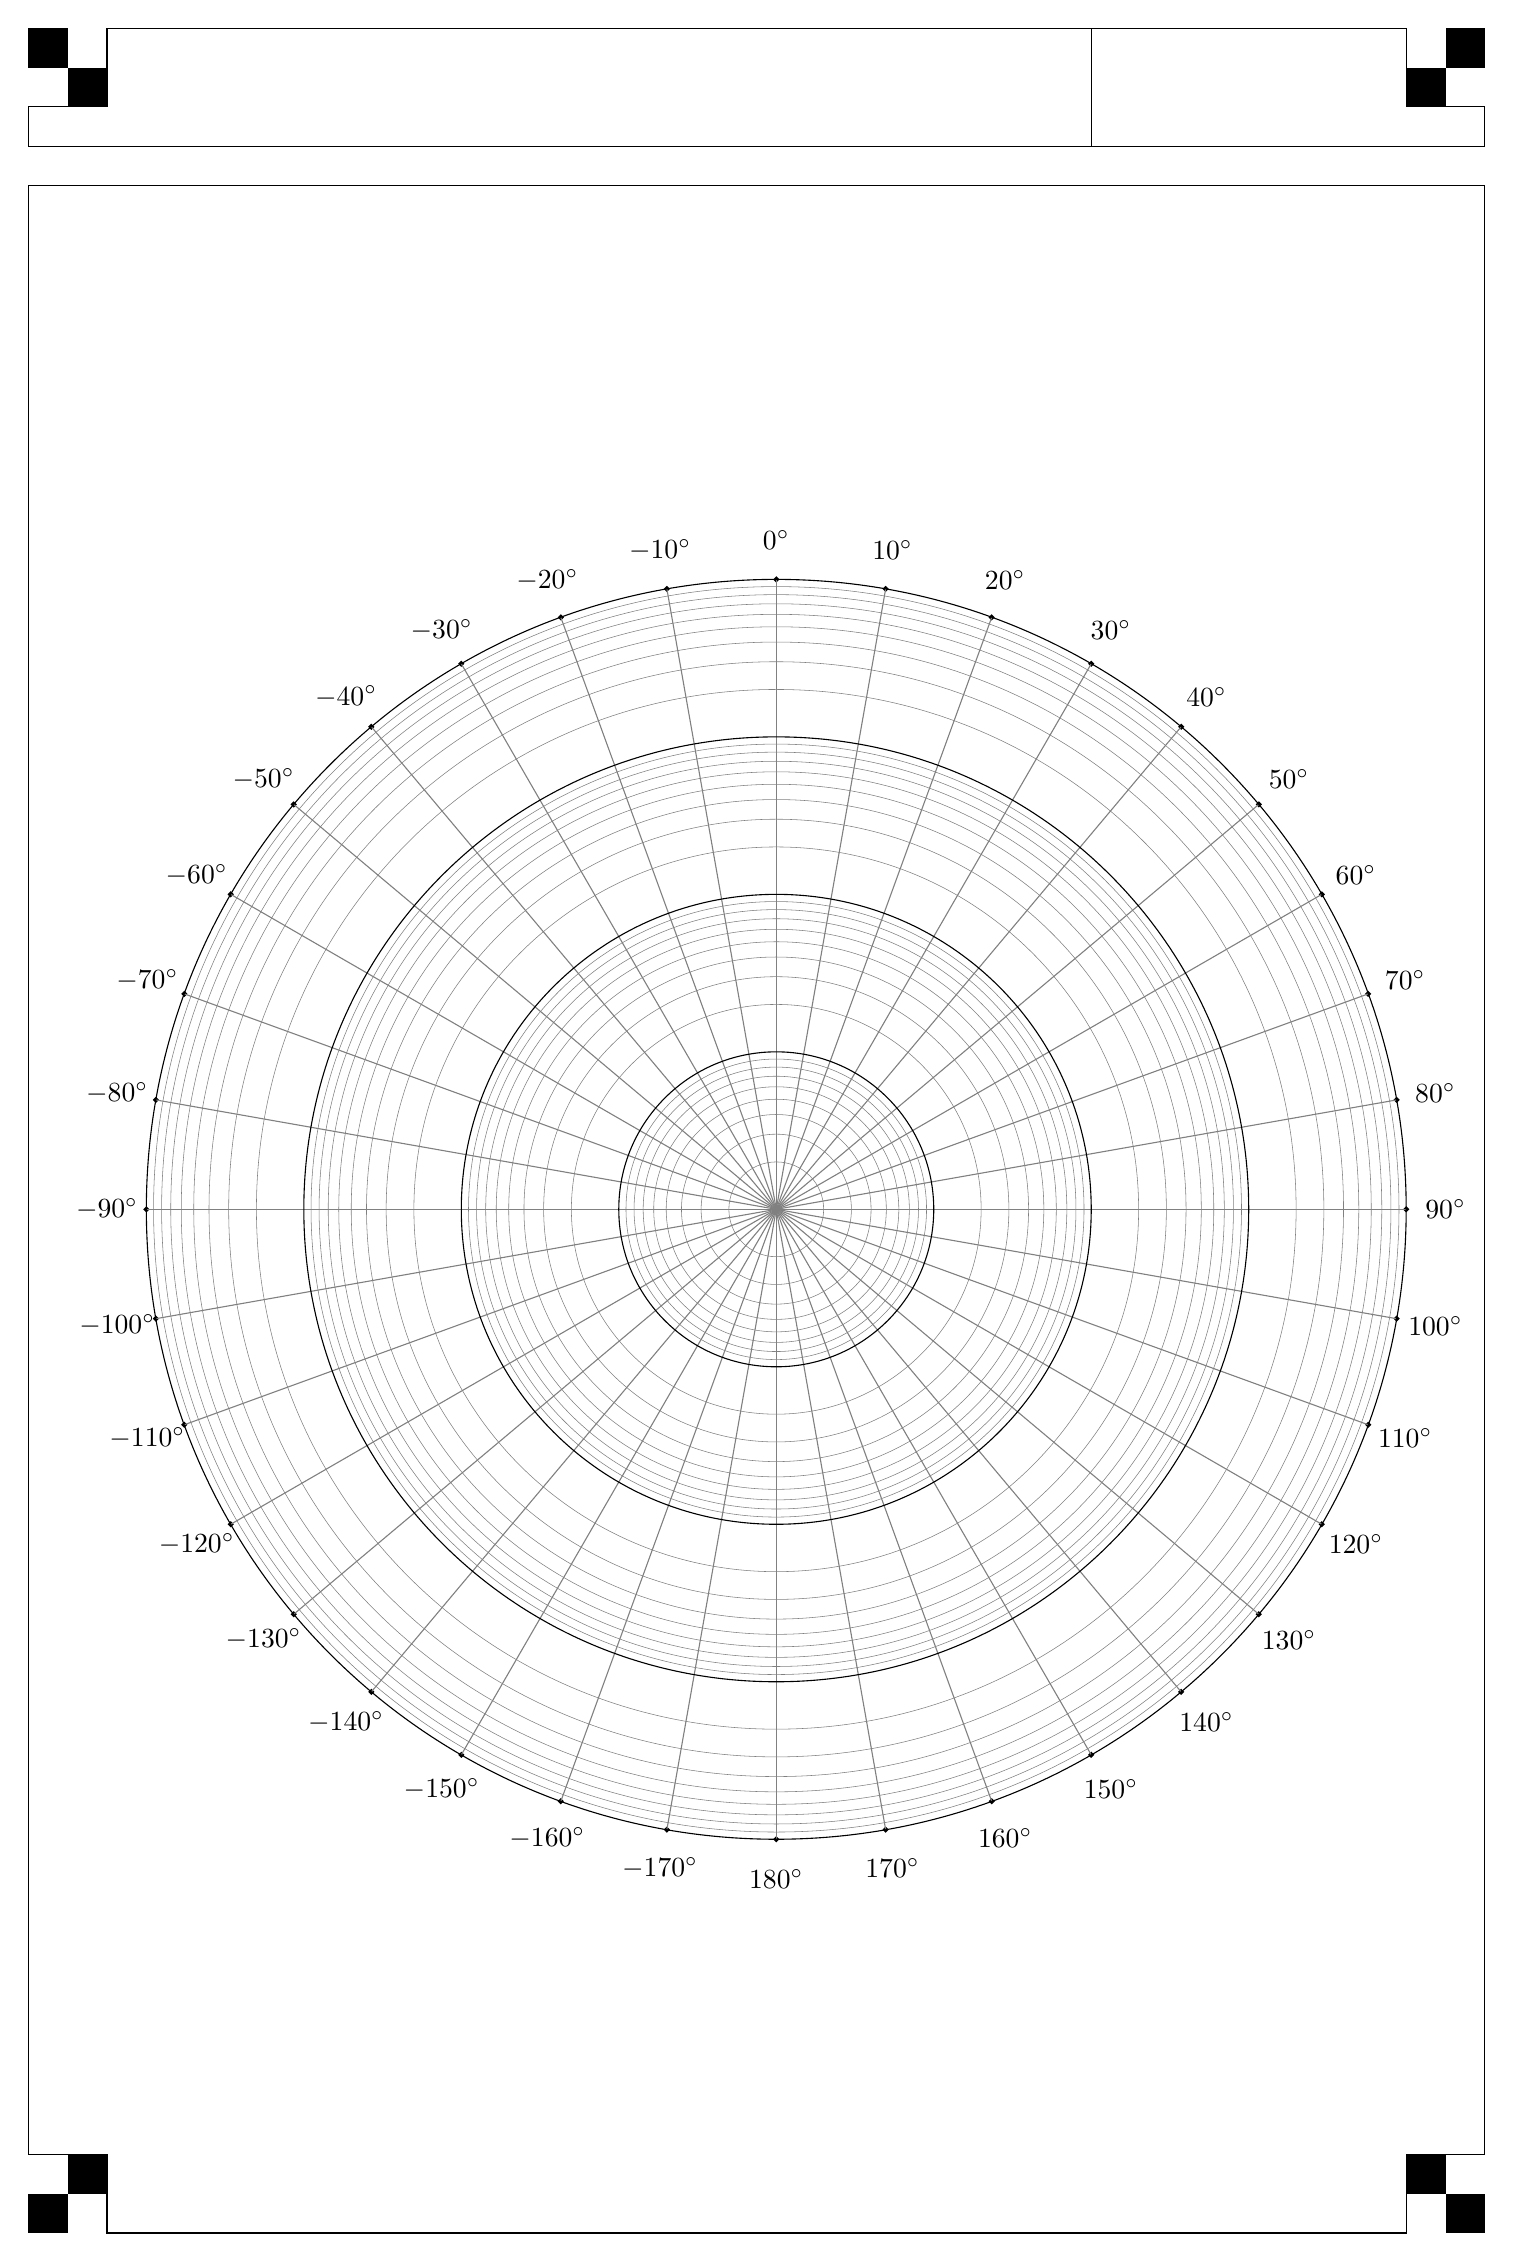
\begin{tikzpicture}
     \fill (0,28) -- (0.5,28) --(0.5,27.5) -- (0,27.5) -- cycle ;
     \fill (0.5,27) -- (1,27) -- (1,27.5) -- (0.5,27.5) -- cycle ;
     \fill (18,28) -- (18.5,28) --(18.5,27.5) -- (18,27.5) -- cycle ;
     \fill (17.5,27.5) -- (17.5,27) --(18,27) -- (18,27.5) -- cycle ;
     \fill (0,0) -- (0.5,0) --(0.5,0.5) -- (0,0.5) -- cycle ;
     \fill (0.5,0.5) -- (1,0.5) --(1,1) -- (0.5,1) -- cycle ;
     \fill (0,0) -- (0.5,0) --(0.5,0.5) -- (0,0.5) -- cycle ;
     \fill (0.5,0.5) -- (1,0.5) --(1,1) -- (0.5,1) -- cycle ;
     \fill (18,0) -- (18.5,0) --(18.5,0.5) -- (18,0.5) -- cycle ;
     \fill (17.5,1) -- (17.5,0.5) --(18,0.5) -- (18,1) -- cycle ;
     \draw (1,28) -- (17.5,28) -- (17.5,27) -- 
           (18.5,27) -- (18.5, 26.5) -- (0,26.5) -- (0,27) -- (1,27) -- cycle;
     \draw (13.5,28) -- (13.5,26.5) ;
     \draw (0,1) -- (0,26) -- (18.5,26) -- (18.5,1) -- (17.5,1) --
           (17.5,0) -- (1,0) -- (1,1) -- cycle ;
\foreach \t in {260,250,...,-90} {
    \draw[thick] ($(9.5,13)+(\t:8)$) circle (0.02) ;
    \draw[thin,gray] (9.5,13) -- ($(9.5,13)+(\t:8)$);

    \coordinate (A) at ($(9.5,13)+(\t:8)$);
    \COPY{\t}{\temp}
    \ADD{\temp}{-90}{\tempa}
    \MULTIPLY{\tempa}{-1}{\tempb}
\node  at ($(A)+(\t:0.5)$)  { $ \tempb^{\circ}$};
}
\foreach \t in {0,1,2,3} {
    \foreach \u in {2,...,9} {
        \draw[gray, line width=0.2pt] 
            ($(9.5,13)+({2.0*(\t+log10(\u))},0)$) 
            arc (0:360:{2.0*(\t+log10(\u))}) ;
    }
    \draw[black, line width=0.4pt] ($(9.5,13)+({2.0*(\t+1)},0)$) arc (0:360:{2.0*(\t+1)}) ;
}
 \end{tikzpicture}
\end{document}
